%Chapter 3

\renewcommand{\thechapter}{3}

\chapter[Data-Driven Likelihood Factorizations]{Improved Data-Driven 
Likelihood Factorizations for Transcript Abundance Estimation
\footnote{This work is presented in the proceedings of ISMB 2017}} 
\label{chapt3}

\section{Introduction}

Shortly after the RNA-seq assay became popular as a tool for transcriptome profiling and 
quantification, the computational community began developing principled inference 
methodologies to allow accurate transcript-level quantification in the presence of 
multi-mapping reads.  Tools such as \cufflinks~\citep{cufflinks}, \rsem~\citep{Li2010RSEM}, 
\mmseq~\citep{Turro2011Haplotype} and \isoem~\citep{Nicolae2011Estimation} provided 
statistical models by which transcript-level abundance estimates could be inferred. 
These methodologies principally rely on maximum likelihood estimation to infer the 
transcript abundances that would be most likely given the observed data (i.e., the 
alignments of the sequenced fragments to the underlying genome or transcriptome). 
Bayesian methodologies such as \bitseq~\citep{bitseq} and \tigar~\citep{tigar} were 
also developed and adopt different inferential approaches varying from fully-Bayesian 
approaches like collapsed Gibbs sampling~\citep{bitseq} to approximate inference 
approaches like variational Bayesian optimization~\citep{tigar,tigar2,bitseqvb}.

These methods vary widely in their details, though adopt a similar 
generative model of the underlying RNA-seq experiment; one which is well-represented 
by the generative model of \rsem~\citep{Li2010RSEM,rsembmc}.  In this chapter, we shall 
refer to this as the \fm.  It is a generative model of an RNA-seq experiment that 
considers the likelihood of observing a collection of alignments as dependent upon 
the parameters of interest (i.e., the transcript abundances), as well as the details 
of each alignment of a sequenced fragment to the reference transcriptome.  In this way, 
the full model provides very high fidelity, and is capable of incorporating a tremendous 
amount of information into the inference procedure (e.g., the implied fragment length 
under each alignment, details about the alignment and the fragment's quality values, 
the probability of different start positions for the sampled fragment, etc.).

Unfortunately, however, this means that straightforward inference procedures that adopt 
this full model scale in the number of considered alignments \emph{per-iteration}.  
For example, a 30 million fragment RNA-seq experiment may produce 100 million fragment 
alignments, all of which are considered by the inference procedure in each of its 
(typically) hundreds to thousands of iterations.  This approach, then, poses two 
problems.  First, inference is typically slow since each iteration must consider 
a large number of independent probabilities.  Second, so as to prevent the inference 
algorithm from becoming even slower, these per-alignment probabilities are typically 
retained in memory, which can lead memory requirements to scale linearly with the 
number of alignments. One approach to mitigate the cost associated with optimizing 
the \fm is to alter the actual inference algorithm that is used.  For example, 
\express~\citep{Roberts2013Express} uses an online-EM algorithm, rather than 
a batch-EM algorithm (by default), to infer transcript abundances.  This eliminates 
the need to cache alignments in memory for efficiency, resulting in constant memory 
usage. However, a single pass over the data is not always sufficient to achieve the 
same accuracy as methods that run batch algorithms to convergence.

One of the more popular approaches for reducing the computational burden and speeding 
up the inference procedure is to form an approximate factorization of the likelihood 
function (see~\Cref{subsec:likelihood}). For example, \mmseq introduced a notion of 
fragment equivalence classes, which treats as equivalent any fragments that align 
to exactly the same set of transcripts.  This leads to a likelihood function in which 
the counts of fragments compatible with subsets of transcripts serve as sufficient 
statistics. The likelihood defined over these counts is typically orders of magnitude 
faster to evaluate, but it can discard certain fragment-level information encoded in 
the alignments. Distinct but related notions of equivalence classes were also 
introduced by~\citet{salzman2011statistical} and \citet{Nicolae2011Estimation}.

Because of the computational economy of this approximate factorization, it 
(or similar variants) were later adopted by new lightweight approaches for 
transcript quantification like \sailfish~\citep{Patro2014Sailfish,Srivastava2016rapmap} 
and \kallisto~\citep{Bray2016Kallisto}.  By coupling a very fast inference approach with 
techniques that removed the requirement of computing traditional alignments for each 
sequenced fragment, such approaches reduced the time required to obtain transcript-level 
quantification estimates by orders of magnitude over existing approaches.  These 
lightweight methods have proven an important and popular development.  Recently, 
\citet{Patro2017Salmon} introduced a new lightweight approach, \salmon, that uses a 
``dual-phase'' inference algorithm, which combines an online stochastic inference method 
with an efficient offline inference algorithm. While adopting a similar approximate 
factorization as \mmseq, \sailfish and \kallisto, \salmon also maintains aggregate 
(i.e., average) weights per equivalence class that allow retaining some information 
about fragment-level probabilities during the offline inference algorithm.  However, this 
information is restricted to a single scalar value per transcript-equivalence class pair, 
and so is necessarily limited in its ability to represent the full model with complete 
fidelity.

In this chapter, we argue that the dual-phase algorithm introduced by \salmon 
allows one to derive a data-driven approximate factorization of the full model 
likelihood function.  The online phase of the algorithm assess each individual 
fragment probability, and uses this information to build a highly-reduced but 
accurate proxy for the \fm likelihood that can be efficiently optimized during 
the offline phase. While only slightly increasing the per-iteration cost of the 
underlying inference algorithm, this data-driven factorization can represent the 
fragment-level likelihood function with much higher fidelity.  In fact, we 
demonstrate that a data-driven likelihood factorization can produce transcript-level 
abundance estimates that display essentially no loss in accuracy compared to what is 
obtained under the full model.  Thus, such a factorization is preferable to the more 
common compatibility-based approximate factorization, since it can provide a substantial 
improvement in accuracy while introducing only a small increase in the computational 
burden.  We note that we focus in this chapter on how to factorize the likelihood function, 
and not, specifically, the algorithm by which this function is best optimized.  Thus, we 
expect the approaches we introduce here to easily translate to other likelihoods or 
optimization approaches; e.g., to variational Bayesian optimizations~\citep{tigar}, or 
natural gradient-based optimization algorithms~\citep{bitseqvb}. Our data-driven 
factorizations are incorporated into the \salmon transcript quantification tool.

%\enlargethispage{12pt}

\section{Approach}

\subsection{The likelihood function and its factorizations}
\label{subsec:likelihood}

We begin by considering the basic generative model laid out
by~\citet{Li2010RSEM}. We consider a transcriptome $T$ to consist of a set of
$M$ transcripts, $t_1, t_2, \dots, t_M$. In a given sample, there are $c_i$
copies of the $i^\text{th}$ transcript. Further, we can assign to each
transcript its length, such that the length of $t_i$ is given by $\ell_i$. The
generative model of an RNA-seq experiment states that the expected number of fragments
sequenced from each transcript type $t_i$ is proportional to the total number of
sequencable nucleotides that it constitutes in the underlying mixture --- that
is we expect that $\alpha_i \propto \eta_i = \frac{c_i \cdot \ell_i}{\sum_j c_j
  \cdot \ell_j}$ --- where $\alpha_i$ is the number of fragments drawn from
transcripts of type $t_i$.  Assuming that each fragment is drawn independently,
the likelihood of a collection $\fragments$ of fragments can be written as:
%
\begin{equation}
  \likelihood{\bm{\theta}; \fragments} = 
  \prod_{f_j \in \fragments} 
  \sum_{i=1}^{M} \Pr\left(t_i \mid \bm{\theta}\right) \Pr\left( f_j \mid t_i \right),
  \label{eqn:likelihood_fm}
\end{equation}
%
where $\bm{\theta}$ denotes the parameters of the model, which are the
underlying transcript abundances. We note that, throughout this manuscript, we
use the term ``fragment'' as a generic term which is represented by a single
read (in single-end protocols) and a read pair (in paired-end protocols). The
methods we propose in~\Cref{sec:methods} work only in terms of the conditional
fragment probabilities, and so are equally-applicable in both single and
paired-end protocols, though the definition of these conditional probabilities
will be protocol dependent.

The primary quantity of interest, with respect to the factorizations being proposed in
this chapter, are the $\Pr\left( f_j \mid t_i \right)$ terms --- that is, the
conditional probability of drawing a particular fragment $f_j$, given transcript
$t_i$. This term encodes, given parameters of the model and experiment, how
likely it is to observe a specific fragment $f_j$ arise from transcript $t_i$.
Many terms can be included in such a conditional probability, some common terms include:
%
\begin{equation}
  \Pr\left( \fraglen{j} \mid f_j, t_i\right) = 
  \frac{\Pr_D\left( \fraglen{j}\right)}{\sum_{k=1}^{\ell_i} \Pr_D\left( k \right)},
  \label{eqn:pr_len}
\end{equation}
%
the probability of observing a mapping of implied length $\fraglen{j}$ for $\frag{j}$ 
given that it derives from $\txp{i}$, where $\Pr_D\left(k\right)$ is the probability of 
observing a fragment of length $k$ under the empirical fragment length distribution $D$;
\begin{equation}
  \Pr\left( p_j \mid \fraglen{j}, f_j, t_i\right) = \frac{1}{\ell_i - \fraglen{j} + 1},
  \label{eqn:pr_start}
\end{equation}
%
the probability of a observing a mapping starting at position $p_j$ for fragment 
$\frag{j}$ given that it has implied length $\fraglen{j}$ and is derived from $\txp{i}$;
\begin{equation}
  \Pr\left( o_j \mid \frag{j}, \txp{i} \right)  = 
      \begin{cases}
    \begin{cases}
      0.5 
    \end{cases}
    & \text{if unstranded}\\
    \begin{cases}
      1.0 & \text{if compatible orientation} \\
      \epsilon & \text{if incompatible orientation}
    \end{cases} &\text{if strand-specific}
      \end{cases},
  \label{eqn:orient}
\end{equation}

the probability of observing a mapping with a specific orientation $o_j$ (i.e., 
forward or antisense) with respect to the underlying transcript for $\frag{j}$, 
given $\txp{i}$, $\epsilon$ (a user-defined constant), and knowledge of the 
underlying protocol, and

\begin{equation}
   \Prob{a_j}{\frag{j}, o_j, \fraglen{j}, p_j, \txp{i}},
  \label{eqn:align}
\end{equation}
%
the probability of observing the particular alignment (e.g., \texttt{CIGAR}
string) $a_j$ for $\frag{j}$ given it is sampled from transcript $\txp{i}$, has
orientation $o_j$, implied length $\fraglen{j}$ and starts at position
$p_j$---such a probability is calculated from a model of alignments, like those 
presented in~\citep{Li2010RSEM,Roberts2013Express,Patro2017Salmon}.

In fact, one can conceive of many such general models of ``fragment-transcript
agreement''~\citep{Patro2017Salmon}. The framework we propose
in~\Cref{sec:methods} can naturally account for such conditional probabilities 
that one might consider as part of $\Prob{f_j}{t_i}$.  However, in this manuscript,
we consider that $\Prob{f_j}{t_i}$ is simply the product of the conditional 
probabilities defined in~\Cref{eqn:pr_len,eqn:pr_start,eqn:orient,eqn:align}, 
appropriately normalized.

\subsection{Equivalence classes and approximate likelihood factorizations}
\label{subsec:eq_classes}

Here, we describe the most common definition of fragment equivalence classes,
and explain how they are used to derive an approximate factorization of the
likelihood function, we adopt a notation similar to~\citet{Patro2017Salmon}.

Let $A\left(\txps, \frag{j}\right)$ be the set of all alignments of fragment
\frag{j} to the transcriptome \txps and let $\mapset{\frag{j}} = \{ \langle i,
\txp{i} \rangle \mid \txp{i} \in A\left(\txps, \frag{j}\right) \}$ be the tuple
of transcripts to which $\frag{j}$ maps---considering the $\txp{i}$ are ordered
by their index $i$. Fragment equivalence classes are defined in terms of the
equivalence relation $\sim$, such that $\frag{m} \sim \frag{n}$ if and only if
$\mapset{\frag{m}} = \mapset{\frag{n}}$. Thus, fragment equivalence classes
consider as equivalent (for the purposes of inference), sequenced fragments that
align to the same set of transcripts. We will refer to $\mapset{\frag{j}}$
as the \emph{label} of $\frag{j}$ for all $\frag{j} \in \eqclass{q}$, where
$\eqclass{q}$ is the equivalence class to which $\frag{j}$ belongs. We will also
refer to $\mapset{\eqclass{q}} = \mapset{\frag{j}}, \forall \frag{j} \in
\eqclass{q}$ as the label of $\frag{j}$'s equivalence class. Finally, it will be
convenient to define the total size of each such equivalence class as
$\eqsize{q} = |\eqclass{q}|$, which is the total number of equivalent fragments
in the class $\eqclass{q}$.

Now, we can write the equivalence class-based approximation to the likelihood function as: 
\begin{equation}
    \likelihood{\bm{\theta};\Frags} \approx 
        \prod_{\eqclass{q} \in \eqclasses}
        \left(\sum_{\langle i, t_i \rangle \in \mapset{\eqclass{q}}} 
        \Prob{\txp{i}}{\bm{\theta}} \cdot \Prob{f}{\eqclass{q},\txp{i}} \right)^{\eqsize{q}},
\label{eqn:likelihood_eq}
\end{equation}
%
where $\eqclasses$ is the set of all equivalence classes, and
$\Prob{f}{\eqclass{q},\txp{i}}$ is the probability of generating a fragment $f$
given that it comes from equivalence class $\eqclass{q}$ and transcript
$\txp{i}$. The key to the efficiency of likelihood evaluation (or optimization)
under this factorization, is that the probability
$\Prob{f}{\eqclass{q},\txp{i}}$ is assumed to be identical for each of the $\eqsize{q}$
fragments in each equivalence class $\eqclass{q}$---hence, we do not
subscript $f$ in~\Cref{eqn:likelihood_eq}. This allows one to replace the
product over all fragments $f_j$ in~\Cref{eqn:likelihood_fm} with a product over
all equivalence classes in~\Cref{eqn:likelihood_eq}. The approximation, of
course, stems from the fact that, under the full model, a fragment $\frag{j}$
may have a probability $\Prob{\frag{j}}{\txp{i}}$ that is arbitrarily different
from $\Prob{f}{\eqclass{q},\txp{i}}$. Moreover, the most common approximations,
like those adopted in \mmseq, \sailfish, and \kallisto consider this
probability to be fixed and essentially independent of any fragment-level
information (e.g., it is set to one divided by the effective
length of $\txp{i}$).

\subsection{What approximate factorizations elide}
\label{subsec:approx_lossy}

\begin{figure}
  \centering
  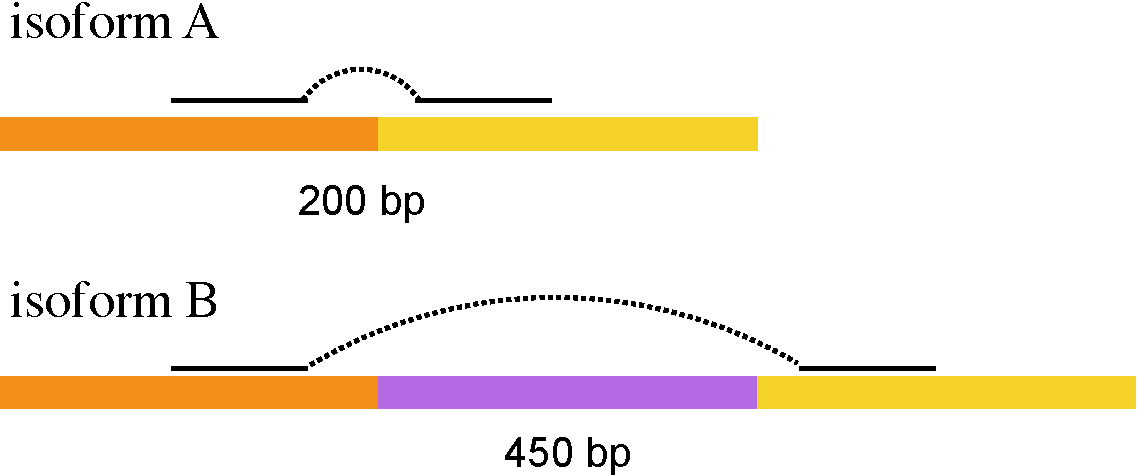
\includegraphics[width=0.4\textwidth, angle=0]{{{Figures/DDFact/Patro.287.fig.1}}}
  \caption[Effect of fragment length on conditional probabilities]
    {A fragment multimapping between two different
    isoforms (A,B) of a gene. Depending on the parameters of the fragment length
    distribution of the underlying sample, either multi mapping locus could be
    more probable \emph{a priori}. Under the approximate likelihood
    factorization that considers only compatibility-based equivalence classes,
    such information is necessarily hidden from the resulting inference
    algorithm. We note that, of course, such multi-mapping can also happen between 
    different genes (e.g., paralogs).}
    \label{fig:len_prob}
\end{figure}

\Cref{fig:len_prob} provides an illustrative example why considering conditional 
fragment probabilities can be important.  Consider a multi-isoform gene, and a 
single fragment $f_j$, which aligns equally well (i.e., the sequence of both ends 
of the fragment match the sequence of the underlying transcripts equally well) to 
isoforms A and B of this gene.  If we consider only transcript-fragment compatibility, 
then both of the alignments illustrated in~\cref{fig:len_prob} are delineated only in 
that isoform A has fewer potential start locations.  However, considering the implied 
length of this fragment, given the expected insert size distribution of the experiment 
(either provided as input to the model, or inferred from the collection of previously 
aligned fragments), can provide strong evidence that one or the other of these isoforms 
was more likely to have generated $f_j$.  For example, were the mean of the fragment 
length distribution $250$, then we would expect isoform A to be much more likely to 
have generated $f_j$.  Conversely, were the mean of the fragment length distribution 
$400$, then we would expect that, in fact, isoform B might have been more likely to 
generate this fragment.  Standard (i.e., compatibility-based) approximate factorizations 
of the full likelihood function into equivalence classes discard (or collapse) this 
fragment-level information.  For example, compatibility-only factorizations of the 
likelihood into equivalence classes simply treat 
$\Pr\left( \fraglen{j} \mid f_j, t_i\right)$ 
as equal for all transcripts in the equivalence class to which fragment $f_j$ belongs. 
The factorization adopted by \salmon attempts to maintain slightly more information by 
computing these conditional probabilities and averaging them; maintaining a single extra 
scalar per transcript-equivalence class pair, that represents the conditional probability 
that any fragment coming from a particular equivalence class would derive from a particular 
transcript.  Though this maintains some extra information, it is not always enough to 
faithfully approximate the full-model likelihood function.

Below, we describe a data-driven approach that allows for a much more faithful 
representation of the \fm likelihood function, while still greatly reducing the 
amount of information that must be maintained for inference.  A broad overview of 
how these factorizations relate to each other is given in~\Cref{fig:tradeoff}, and 
the specific factorizations are described in more detail below.

\begin{figure}
  \centering
  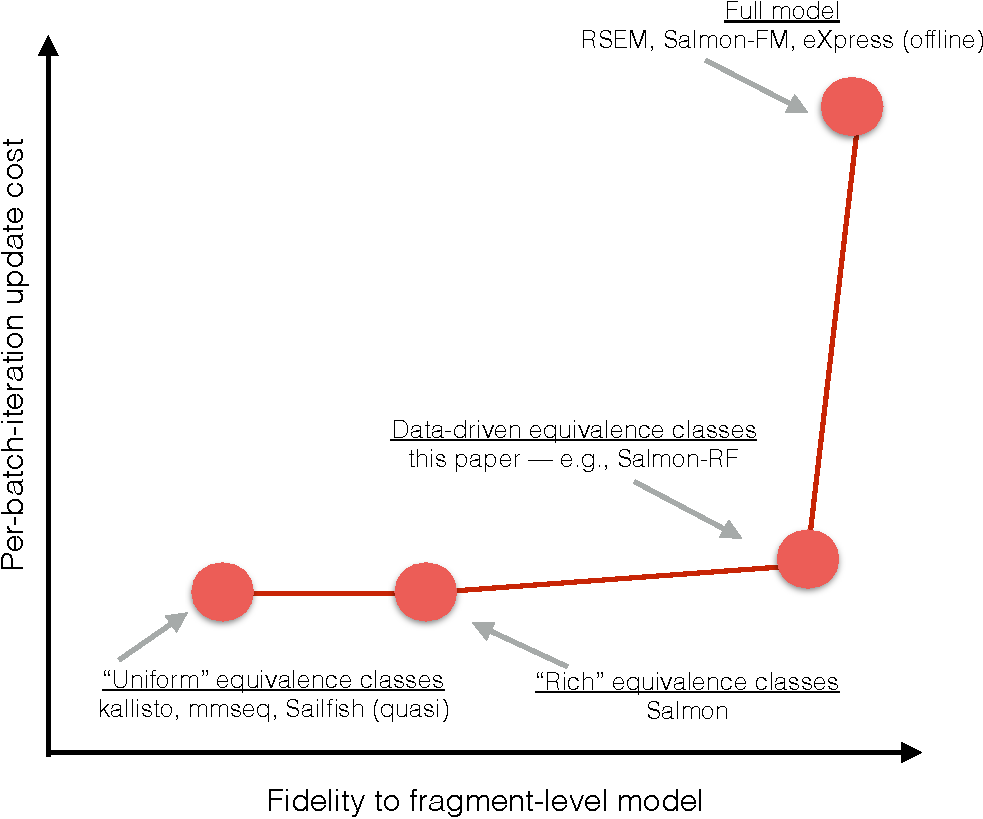
\includegraphics[width=0.6\textwidth]{{{Figures/DDFact/Patro.287.fig.2}}}
  \caption[Tradeoff between the computational efficiency and the inference technique]
    {There is a conceptual tradeoff between the
    computational efficiency of an inference technique, and the fidelity with
    which it models the full, fragment-level likelihood function. \kallisto,
    \sailfish (using quasi-mapping~\citep{Srivastava2016rapmap}) and \mmseq
    simply consider the compatibility of fragments with transcripts, and thereby
    discard the conditional fragment-level probabilities completely. \salmon
    collapses the fragment-level conditional probabilities to a single scalar
    (their average value) per-equivalence class; this recovers some of the
    fidelity lost in the other approaches, but can still discard useful
    fragment-level information. Approaches that consider each fragment
    independently in each round of the optimization algorithm (e.g. \rsem and
    \salfm and \express (offline)) sacrifice no fidelity, but each iteration
    scales with the total number of aligned / mapped fragments. Our proposed
    data-driven clustering approach (\salrf) captures most of the important
    fragment-level probabilities of the \fm, while retaining an update time very
    similar to \salmon's standard model in its offline rounds. The online rounds
    of \salmon and \express are not directly comparable to the batch rounds
    considered in this figure (they update the parameters more frequently), but
    they do consider the conditional probability of each fragment
    individually.}
    \label{fig:tradeoff}
\end{figure}

\section{Methods}
\label{sec:methods}

As illustrated in~\Cref{fig:tradeoff} and described above, the approximations
that rely on \cb factorizations can discard information that may be
useful for correct transcript abundance estimation. Specifically, such
notions of equivalence classes sacrifice per-fragment information encoded in the
conditional probabilities $\Prob{\frag{j}}{\txp{i}}$. We propose here alternative 
notions of equivalence classes that take into account both the transcripts with 
which a fragment is compatible, as well as the vector of conditional probabilities 
that encodes how likely the fragment is to have been sequenced from each such 
transcript. That is, these factorizations account both for the set of transcripts 
$\txp{1}, \dots, \txp{k}$ to which a fragment $\frag{j}$ maps, as well as the conditional
probabilities $\Prob{\frag{j}}{\txp{1}}, \dots, \Prob{\frag{j}}{\txp{k}}$ that
$\frag{j}$ was sampled from each of these transcripts. Our approach is agnostic
to how $\Prob{\frag{j}}{\txp{i}}$ is computed, but, as stated
in~\Cref{subsec:likelihood}, we consider here each conditional probability to be the
product of \Cref{eqn:pr_len,eqn:pr_start,eqn:orient,eqn:align}, appropriately
normalized.We accomplish this by defining new equivalence relations over
fragments that consider and summarize these conditional probabilities in a
data-driven manner.

As one divides each equivalence class into smaller sub-classes of fragments, the
factorized likelihood approaches the likelihood (and hence fidelity) of the \fm.
Conversely, as the number of equivalence classes increases so does the
complexity of evaluating and optimizing the likelihood.

Here, we introduce two different factorization methods that refine the \cb
notion of equivalence classes. These approaches are a refinement in the strict
sense that each sub-cluster of fragments that fall within the newly-defined
equivalence classes align to the same set of transcripts as all other fragments
in the original, \cb definition of the equivalence class. However, in these
factorizations, the conditional fragment probabilities (with respect to the set
of transcripts) tend to exhibit smaller distance to mean; i.e., the approximate weight
used to summarize the conditional probability of all fragments within these
refined equivalence classes is much closer to the individual conditional
probabilities of all the fragments placed in the class. Subsequently, this
leads to a more accurate approximation of the likelihood function.
Moreover, we find that only a small number of such refined equivalence classes
is required to approximate the full likelihood very closely, meaning that the
computational complexity of evaluating and optimizing the likelihood function is
very close to what is required when considering the original \cb equivalence class
factorization (\cref{tab:performance_table}).
% \begin{table}[h]
	% \end{table}
\subsection{Rank-based factorization}
\label{subsec:rank_fact}
We call the first factorization method that we consider to refine the notion of
equivalence classes the ``rank-based factorization''. We consider all
transcripts to which a fragment aligns, and sort the transcripts based on the
conditional probability values of the fragment given each transcript. Then, the
equivalence class for a fragment is determined by the set of transcripts to
which it maps, \emph{and} the rank-order of the conditional probabilities for
this fragment given those transcripts. For instance, consider \num{1000}
fragments which all align to the transcripts $t_1$ and $t_2$, where $250$ of
these fragments align to $t_1$ with a higher conditional probability than that
with which they align to $t_2$ (and vice-versa for the rest). In this case, the
rank-based equivalence relation will induce 2 equivalence classes (whereas the
\cb relation would have induced 1), the first $250$ fragments will become
members of one equivalence class with label $\{\tup{1}{1} , \tup{2}{2}\}$ and the rest
will be assigned to another equivalence class with the label 
$\{ \tup{1}{2} ,\tup{2}{1} \}$.
As with the original notion of \emph{rich} equivalence classes in
Salmon~\citep{Patro2017Salmon}, a single scalar value per transcript is saved in
each equivalence class, which is the mean of all conditional probabilities of the
fragments given each transcript. Of course, in this factorization, the total
number of equivalence classes is typically larger than the number of \cb
equivalence classes. Formally, we define the rank-based equivalence relation
$\sim_{<}$ as follows: let $r\left(f, \{\tup{i_1}{i_1}, \tup{i_2}{i_2}, \dots,
\tup{i_j}{i_j}\}\right)$ be a function that returns a permutation $\sigma$ of
$\left(\txp{i_1}, \txp{i_2}, \dots, \txp{i_j}\right)$ such that
$\Prob{f}{\txp{\sigma_1}} \le \Prob{f}{\txp{\sigma_2}} \le \dots \le
\Prob{f}{\txp{\sigma_j}}$, with ties broken arbitrarily in favor of the
transcript having the smaller index. We define two fragments $\frag{m}$ and
$\frag{n}$ to be equivalent ($\frag{m} \sim_{<} \frag{n}$) if and only if
$\mapset{\frag{m}} = \mapset{\frag{n}}$ and $r\left(\frag{m},
\mapset{\frag{m}\right)} = r\left(\frag{n}, \mapset{\frag{n}\right)}$.
%
\begin{figure}[t!]
\centering
  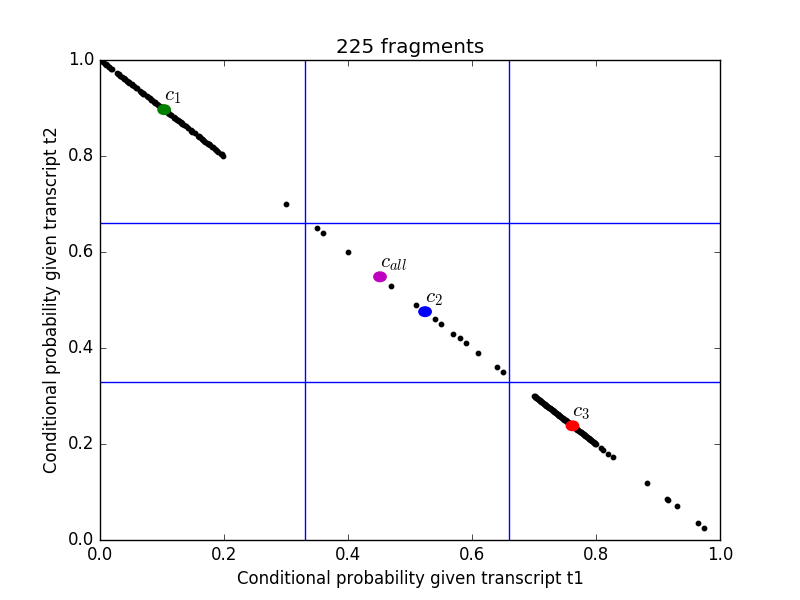
\includegraphics[width=0.7\textwidth, angle=0]{{{Figures/DDFact/Patro.287.fig.3}}}
  \caption[Visualization of factorizing an equivalence class]{\label{fig:rangefactor} 
  Factorizing an equivalence class consisting of 225 fragments and 2 transcripts into k=3 
  bins. Each dot represents one fragment. The vertical lines indicate borders of bins for 
  transcript $t_1$ and the horizontal lines show borders of bins for transcript $t_2$. 
  The purple circle with label $c_{all}$ shows the center for original equivalence class. 
  The rest of the circles are indicators of the centers for each cluster after the 
  factorization.}
\end{figure}
%
\subsection{Range-based factorization}
\label{subsec:range_fact}
We consider a second factorization approach that we call ``range factorization'' 
(\salmonrf).  In this approach, we seek equivalence classes that have fragments which 
both align to the same set of transcripts \emph{and} which have similar conditional 
probabilities with respect to these transcripts. To motivate this approach, consider, 
first, the case of two fragments that have exactly the same conditional probabilities 
for the same set of transcripts, then one can safely group them together without any 
loss of accuracy with respect to the original likelihood function. In fact, this is 
the equivalence relation proposed by~\citet{Nicolae2011Estimation}. However, this 
particular factorization can have a negative impact on performance since most of the 
time probabilities of fragments are not exactly proportional. Hence, this can lead to 
a model similar to the full model that considers all fragment-transcript likelihood 
values. However, we can compromise the ``exact'' proportionality of probabilities for 
the sake of performance. Instead of clustering fragments that have exactly proportional 
probabilities, we place fragments with the same conditional probability ``range'' into 
the same equivalence class. We first divide the valid range of probabilities 
$\left[0,1\right]$ into $k$ bins, and then consider two conditional probabilities equal 
if their values are in the same bin. Two fragments are considered equivalent under this 
definition, denoted $\sim_{r}$, if they fall into the same set of bins with respect to 
all transcripts to which they align.  Formally, let 
$b_k\left(f, \{ \tup{i_1}{i_1}, \tup{i_2}{i_2}, \dots, \tup{i_j}{i_j}\}\right)$ be a 
function that returns a vector of bin values (one for each transcript, and each between 
$0$ and $k-1$).  We define two fragments $\frag{m}$ and $\frag{n}$ to be equivalent 
($\frag{m} \sim_{r} \frag{n}$) if and only if $\mapset{\frag{m}} = \mapset{\frag{n}}$ and 
$b_k\left(\frag{m}, \mapset{\frag{m}\right)} =  b_k\left(\frag{n}, \mapset{\frag{n}\right)}$.

We can tune the parameter $k$ to tradeoff of the number of such equivalence classes versus 
the accuracy they provide. As $k$ approaches infinity (or, rather, machine precision), the 
fidelity provided by this factorization approaches that of the full model, because all 
fragments will end up in either single-member equivalence classes, or in equivalence classes 
of fragments having conditional probabilities exactly proportional to theirs. On the other 
hand, as $k$ gets smaller, the number of clusters gets closer to a small constant times the 
number of \cb equivalence classes, but each cluster consists of fragments with the wider 
range of conditional probabilities.  In this approach, we do not simply replace each 
conditional probability with the center of the bin into which it falls.  Rather, for 
each bin, we record the sum and a total number of conditional probabilities stored in 
this bin.  After processing all fragments, the centroid of each bin is computed and used 
as the representative conditional probability for this bin.  This model is a natural 
extension of the rich equivalence class model used in \salmon, and the models coincide 
when $k = 1$. Throughout this chapter, range-based equivalence classes have a number of 
bins equal to $4 + \ceil{\sqrt{\left|\mapset{\eqclass{q}}\right|}}$. 

\Cref{fig:rangefactor} provides a good example of this factorization and its impact on 
the average of conditional probabilities for each transcript. There are 225 fragments 
that all are aligned to the two transcripts in this equivalence class. Each dot represents 
a fragment with its $x$ value equal to $\Prob{f}{t_1}$ and $y$ value equal to 
$\Prob{f}{t_2}$. $c_{\text{all}}$ shows the average value of conditional probabilities 
of all fragments for transcript $t_1$ and $t_2$. As can be observed, the deviation of 
$c_{\text{all}}$ from many of the conditional probabilities is large since the conditional 
probabilities are widely distributed over the range from zero to one. However, when we 
divide the range into three bins and then separate fragments based on the bin into which 
their conditional probabilities fall, we obtain three clusters containing fragments whose 
within-cluster conditional probabilities fall into much smaller ranges. So, in this case, 
all fragments that have the same bin for their conditional probability given $t_1$ and 
their conditional probability given $t_2$ end up in the same cluster. Lines show the 
borders of each bin and colored circles show the centroids used to represent the conditional 
probabilities in each bin. In this case, we expect to obtain results closer to the \fm; yet, 
the number of clusters over which one must iterate to apply the EM algorithm is sill much 
smaller than the total number of fragments (see~\Cref{tab:performance_table}).

Though we have implemented and experimented with both of these alternative factorizations, 
in this results of this chapter we will focus on the \rangebased factorization, as we observe that it almost 
always provides a better approximation of the likelihood than the \rankbased factorization.

\section{Results}
\label{sec:results}

We test the ability of our proposed factorization to improve the approximation
of the \fm likelihood on both synthetic and experimental data. We demonstrate
that, as expected, the \rangebased factorization almost always provides a very
good approximation of the \fm likelihood. Interestingly, we also observe that it
sometimes leads to a slightly more accurate solution than when no factorization
is applied (i.e., when the likelihood is evaluated for each fragment
independently). Though we have not investigated this in depth, it is likely
that, in some cases, a small degree of smoothing of the conditional
probabilities can lead to a more stable and accurate solution.

We consider both small-scale and transcriptome-wide simulated data.
In~\Cref{res:smallscale} we consider simulations over the transcripts from
families of paralogous genes. Such situations represent the most challenging
abundance estimation problems for transcript quantification tools since high
levels of multi-mapping are prevalent. We conduct the simulations over many
random settings of the abundances of these transcripts, and look at how well
different methods are able to recover the true abundances at different average
coverage levels. We directly observe how, in the most adversarial situations,
the proposed factorization allows us to recover important information that leads
to improved abundance estimates.

In~\Cref{res:largescale} we explore the effect that different factorizations
have on abundance estimates transcriptome-wide. Here, we observe that, while the
data-driven factorizations lead to improved abundance estimates, the differences
between methods becomes much smaller, since the statistics are aggregated over
the entire transcriptome and since many transcripts fall into the ``easy'' case
of abundance estimation. The differences between methods, while still moderate,
are larger when we restrict our assessment to a more difficult subset of transcripts.

Finally, in~\Cref{res:expdata}, we examine the effect of different factorization
methods over experimentally sequenced data. We explore how closely different
factorizations approach the abundance estimates derived by \rsem---though we note
(as observed in some of the simulated data) that \rsem is not necessarily more
accurate than the alternative methods or factorizations.

\begin{figure}
  \centering
  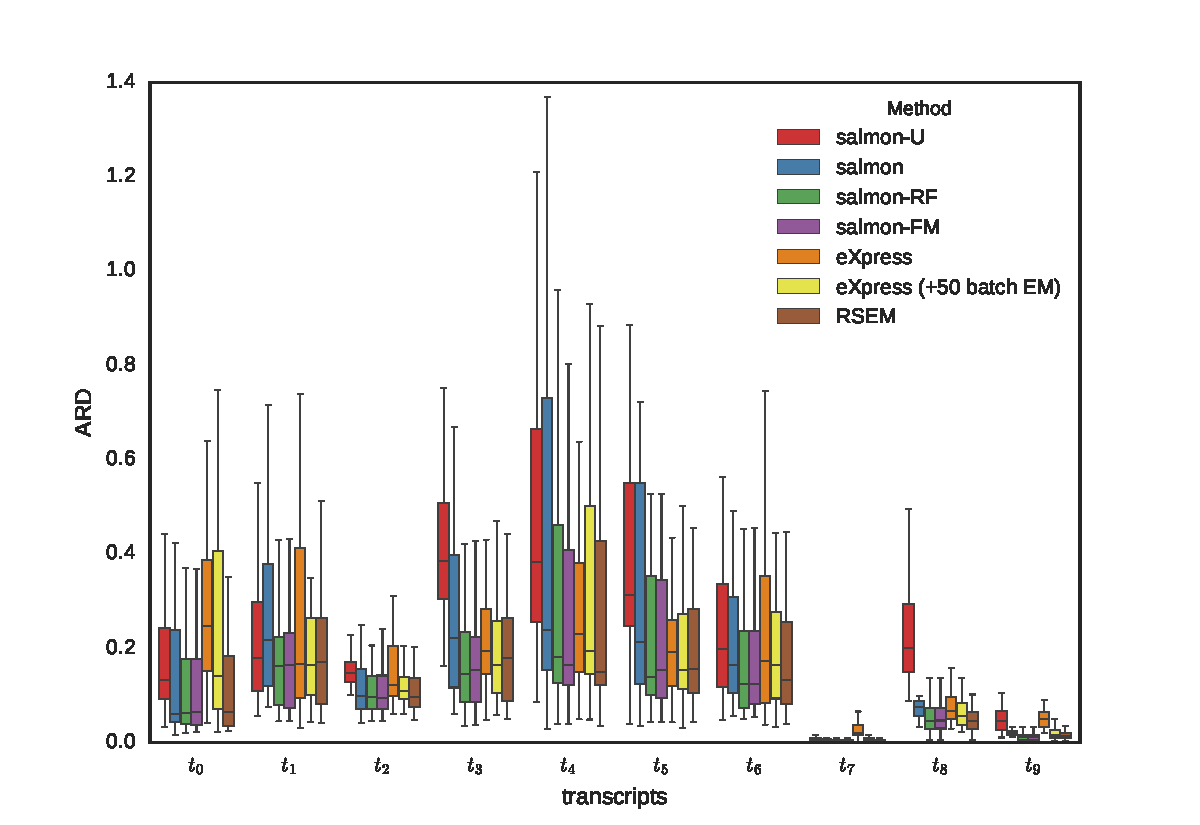
\includegraphics[width=0.3\textwidth, height=3.5cm]{{{Figures/DDFact/Patro.287.fig.4a}}}
  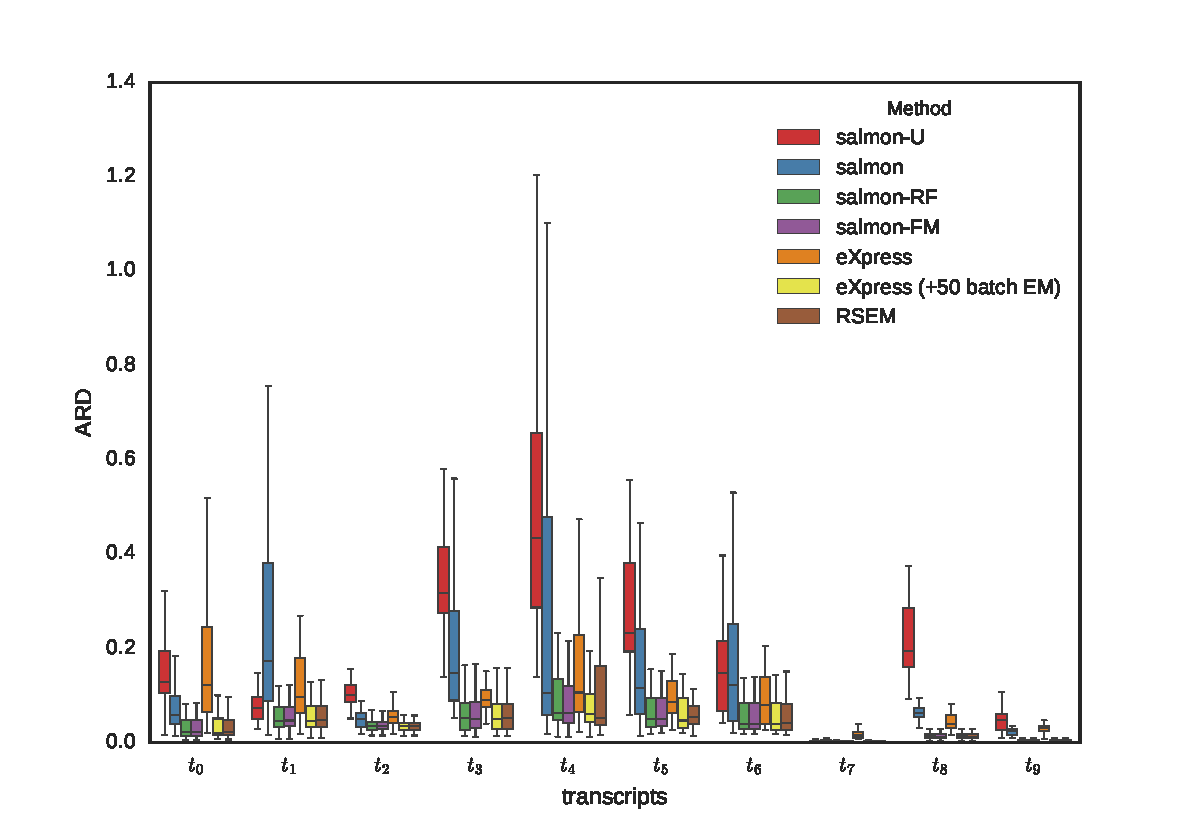
\includegraphics[width=0.3\textwidth, height=3.5cm]{{{Figures/DDFact/Patro.287.fig.4b}}}
  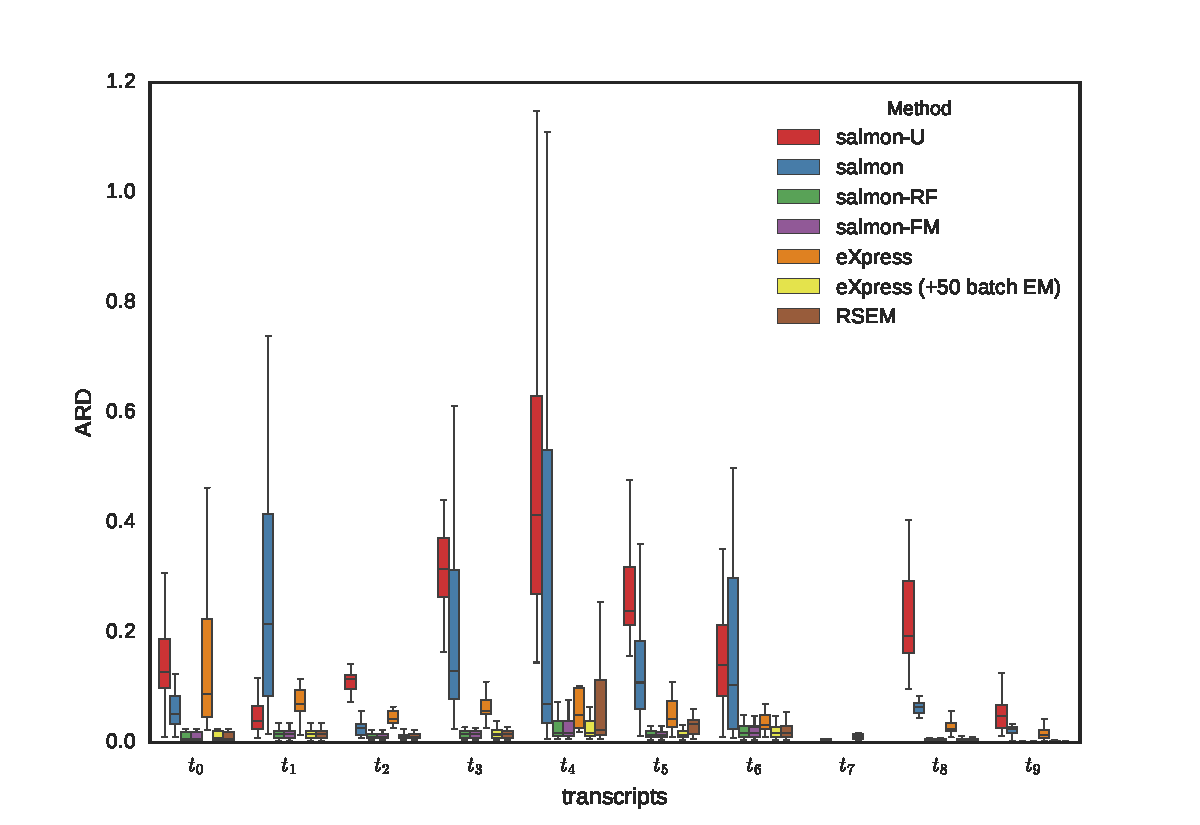
\includegraphics[width=0.3\textwidth, height=3.5cm]{{{Figures/DDFact/Patro.287.fig.4c}}}
  \caption[Comparing quantifications of isoforms of paralog genes - \gene{RAD51}]
  {Applying different methods of transcript abundance estimation in alignment mode on 
  two sets of data in 3 depth of fragment sequencing. Top (a) are all isoform transcripts 
  of gene \gene{RAD51}. The bottom (b) is from transcripts of four different paralogs of 
  \gene{RAD51}, \gene{RAD51B},\gene{RAD51C}, \gene{RAD51D}. In each row the left most 
  plot refers to  experiment with counts of 1X coverage, the middle one to 10X and the 
  most right plot refers to the experiment with fragment counts of 100X coverage.
  Distribution of ARDs on isoforms of \gene{RAD51}.}
  \label{fig:rad51}
\end{figure}
\begin{figure}
  \centering
  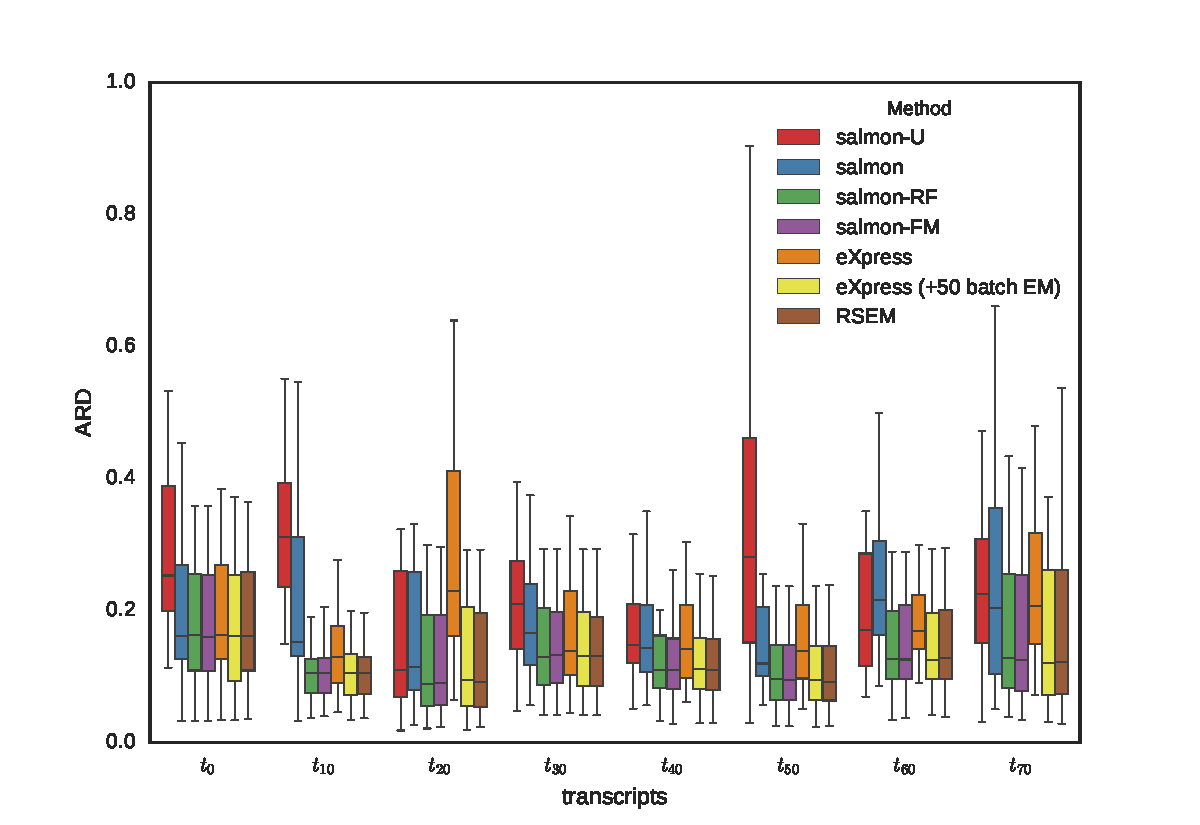
\includegraphics[width=0.3\textwidth, height=3.5cm]{{{Figures/DDFact/Patro.287.fig.4d}}}
  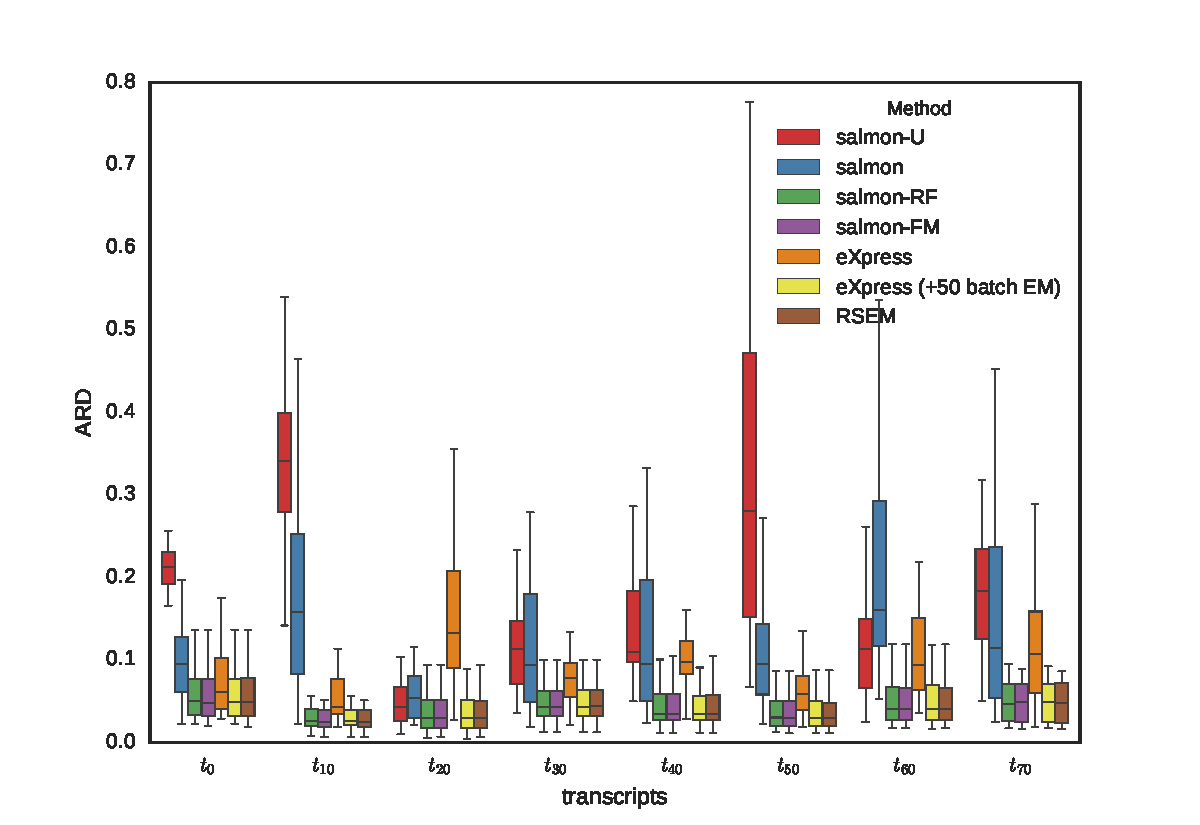
\includegraphics[width=0.3\textwidth, height=3.5cm]{{{Figures/DDFact/Patro.287.fig.4e}}}
  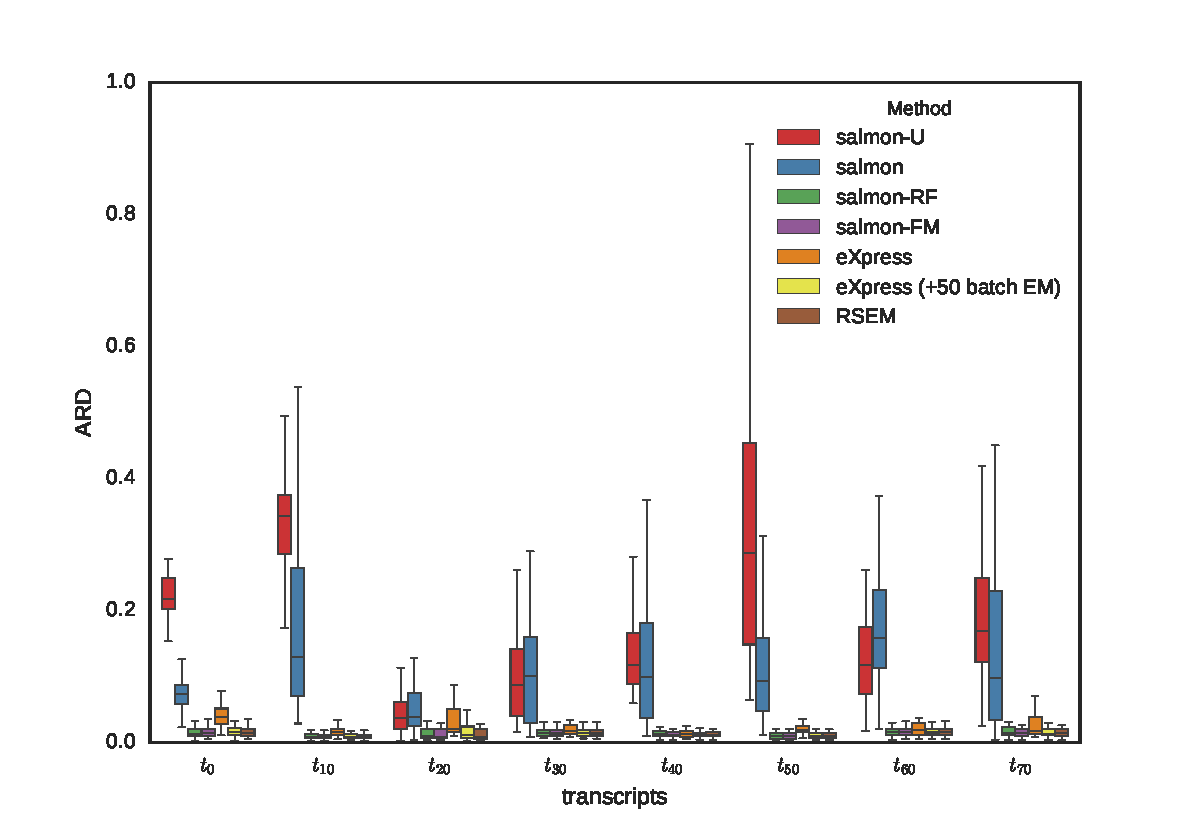
\includegraphics[width=0.3\textwidth, height=3.5cm]{{{Figures/DDFact/Patro.287.fig.4f}}}
  \caption[Comparing quantifications of isoforms of paralog genes - 
  a family of 4 \gene{RAD51} paralogs.]
  {Applying different 
  methods of transcript abundance estimation in alignment mode on two sets of data in 
  3 depth of fragment sequencing. Top (a) are all isoform transcripts of gene \gene{RAD51}. 
  The bottom (b) is from transcripts of four different paralogs of 
  \gene{RAD51}, \gene{RAD51B},\gene{RAD51C}, \gene{RAD51D}. In each row the left most 
  plot refers to experiment with counts of 1X coverage, the middle one to 10X and the 
  most right plot refers to the experiment with fragment counts of 100X coverage.
  Distribution of ARDs on isoforms of a family of 4 \gene{RAD51} paralogs.}
  \label{fig:rad51genes}
\end{figure}

%%
% Explain why alignment and not mapping.
%%
In~\Cref{res:smallscale,res:largescale,res:expdata} we consider the transcript
abundance estimates generated by \rsem, \express (both in default mode and with 
50 batch EM rounds) and variants of \salmon (using different factorizations). 
We focus on the performance of these tools when quantifying
abundances using alignments, instead of mappings~\citep{Srivastava2016rapmap}.
We keep the input data as close as possible, since the purpose of this chapter is
not an investigation of the effect of alignment versus mapping on expression
estimation, but rather the effect of the factorization of the likelihood and how
that factorization affects inference. We noticed that, regardless of the
factorization used, there was a small but persistent gap between non-alignment-based
tools (\kallisto and mapping-based variants of \salmon) compared to \rsem and 
alignment-based variants of \salmon on the \rsemsim data. It is not clear that 
this is due to any fundamental superiority of alignment compared to mapping, 
but rather, may be a result of the fact that the specific error model, learned 
by \rsem and used to simulate reads in \rsemsim, acts as a ``side-channel'' of 
information for alignment-based approaches.  However, this question, though 
outside the scope of this work, deserves further consideration and analysis.

% In the supplementary material, we explore the effect of these factorizations on
% mapping-based solutions by comparing different variants of mapping-based \salmon
% with \kallisto (which only allows using pseudoalignment for quantification).

\paragraph{Alternative factorization variants:} \salmon (i.e., without any
modification) uses a \cb notion of equivalence classes called ``rich''
equivalence classes. Under this notion, the equivalence classes themselves are
\cb, but each transcript-equivalence class pair is associated with a scalar
weight which is computed as the mean conditional probability of all fragments in
this equivalence class to derive from this transcript. We also consider a
variant of \salmon (denoted as \salmonu herein) that adopts a purely \cb notion
of equivalence classes. That is, it stores no extra information about the
conditional probability of deriving the fragments in each equivalence class from
the different transcripts, and during inference considers only that $\Prob{f}{t}
= \Prob{p}{f,t} = 1 / \elength{t}$, where $\elength{t}$ is the effective length
of transcript $t$ and is defined as $\elength{t} = \length{t}-
\mu_d^{\length{t}}$. $\mu_d^{\length{t}}$ is the mean of the truncated empirical
fragment length distribution as described in~\citep{Patro2017Salmon}.

We also consider a variant of \salmon, \salmonfm, that performs no additional
factorization. Instead, like \rsem, it considers each fragment and its relevant
conditional probabilities independently. In this case, the only difference
between \salmonfm and \rsem is that the former computes the conditional fragment
probabilities using an \emph{online} stochastic inference algorithm, while \rsem 
recomputes the conditional fragment probabilities after updating auxiliary model 
parameters during the first 10 iterations of an offline (i.e., batch) EM procedure.

Finally, we consider a variant of \salmon, \salmonrf, that uses the
range-factorization described in~\Cref{subsec:range_fact} to generate
equivalence classes based on $\sim_{r}$ and compute the associated weights.

We use both the mean absolute relative difference (MARD) and Spearman correlation
to assess performance.  We define the absolute relative difference (ARD) as:
%
\begin{equation}
\label{eq:ard}
  \text{ARD}_i =
  \begin{cases}
    0                                            & \text{ if } x_i + y_i  = 0 \\
    \frac{\left|x_i - y_i\right|}{ \left(x_i + y_i\right)} & \text{ otherwise }
  \end{cases},
\end{equation}
%
Where $y_i$ is the estimated number of reads originating from $\txp{i}$ and $x_i$ is 
the true (or assumed) number of reads originating from $\txp{i}$. The MARD is simply 
defined as $\text{MARD} = \frac{1}{M} \sum_{i=1}^{M} \text{ARD}_i$, where $M$ is the 
total number of transcripts.

\paragraph{Experimental setup and software parameters:}
In the tests below, \salmon v0.8.0 was run in alignment mode with the
\texttt{--useErrorModel} flag. \salrf consists of \salmon run with
\texttt{--useRangeClusterEqClasses 4}. \salu consists of \salmon run with
\texttt{--noRichEqClasses}. \rsem v1.3.0 was run with default parameters.
\express v1.5.1 was run with \texttt{--no-bias-correct} and other parameters
were left as default (the extra parameter \texttt{--additional-batch 50} was
used to produce the \expressEM results). All alignments were generated using
\emph{Bowtie 2} version 2.2.9 with the default parameters chosen by \rsem. We
note that these default parameters disallow indels in the resulting alignments
(though \salmon and \express allow indels in the alignments the process, \rsem
does not). Further, we note that since we examine simulated data without bias
and since we compare against \rsem (which does not model sequence-specific or
fragment-GC bias) in the experimental data, we run all other methods without
bias correction. On experimental RNA-seq data, one might expect bias correction
alone to substantially improve the accuracy of a given method. Though those
accuracy improvements should be orthogonal to those obtained by improving the
fidelity of the likelihood function. All the tests are performed on a 64-bit
Linux server with 256GB of RAM and 4 x 6-core Intel Xeon E5-4607 v2 CPUs running
at 2.60GHz.


\subsection{Small-scale simulations on \gene{RAD51} and its paralogs}
\label{res:smallscale}
We first consider a few small-scale simulations to motivate how the conditional
probabilities considered by the \fm (and approximated closely by the \rangebased
equivalence classes) might improve abundance estimates. We note that these
simulations are specifically constructed to represent adversarial and
difficult-to-quantify mixtures of highly related isoforms. We consider the
transcripts from large families of paralogous genes, under many random
distributions of abundances. Often, the fragments will align to many different
transcripts with few-or-no nucleotide differences, and sometimes even with
similar implied insert sizes. Thus, we expect that closely approximating the
conditional fragment probabilities might have a large effect in this case. We
note, however, that such adversarial abundance configurations are likely rare in
experimental data.

We consider two different, small-scale tests focusing around the gene
\gene{RAD51} and members of its paralogous family in \emph{Homo Sapiens}. 
The \gene{RAD51} family includes eight paralogous genes including
\gene{RAD51} itself. \gene{RAD51} codes for a $339$-amino acid protein that has
a significant role in repairing double strand breaks of DNA~\citep{yates2015ensembl}.

In the first experiment we apply \rsem and all varieties of \salmon on all
isoforms of the \gene{RAD51} gene. We extracted all (10) reference transcripts of
\gene{RAD51} from the Ensembl (release 80) reference transcriptome. True reads
counts for all transcripts were generated by sampling a read count for each
transcript uniformly over $\left[1,200\right]$; these counts represent base-depth
coverage (left) in~\Cref{fig:rad51}.  These counts were multiplied by $10$ to
derive the input read counts at $10X$ coverage (\Cref{fig:rad51}, center) and
by $100$ to derive the counts at $100X$ coverage (\Cref{fig:rad51}, right).

Given these read counts, the Polyester simulator~\citep{frazee2015polyester} was
then used to simulate $5$ different read sets (replicates) from the same input
distribution. This entire procedure was repeated $30$ times, setting 
\texttt{R}'s random seed from $1$ to $30$ in sequence.

Since the reads are simulated, we can assess the deviation of the estimated
abundances from the exact abundances for each transcript. We use the absolute 
relative difference (ARD) of estimated versus true read counts
(\Cref{eq:ard}) as the metric to evaluate the accuracy of different methods for
each transcript over replicates, and~\Cref{fig:rad51} shows a box plot of the
distribution of ARD values over the $30$ simulations.

As we expect, \salmonu generally yields the largest ARDs, failing to utilize the
information contained in the conditional fragment probabilities. \salmon
generally performs better, suggesting that, even in this complex scenario, the
aggregate weight maintained in the rich equivalence classes helps to recover
some (but not all) of the fidelity of the full model. However, \salmonrf, while
only slightly increasing the number of equivalence classes considered, produces
ARDs very close to those of \rsem, \expressEM and \salmonfm. This suggests that, even in
this adversarial scenario, the \rangebased equivalence classes allow us to
recover the inferential accuracy of the \fm.

To further explore difficult abundance estimation scenarios, we consider the
case of the presence of high abundance isoforms from more than one gene in the
reference. Therefore, in the second set of experiments we consider 4 paralogs of
\textit{RAD51} (\gene{RAD51}, \gene{RAD51B}, \gene{RAD51C} and \gene{RAD51D}).
We extract all transcripts corresponding to these genes and we run the same
simulation as above with respect to all of these transcripts. Evaluation of ARDs
for every transcript in all genes is displayed in~\Cref{fig:rad51genes}. The
results in this case are similar to what was observed in the single gene
experiment. In some cases, like transcript \gene{ENST00000553595} from
\gene{RAD51B} (which is displayed as $t_{10}$ in~\Cref{fig:rad51genes}), both
\salu and \salmon fail to estimate an accurate abundance. In other cases \salmon
performs better than \salmonu, e.g., transcript \gene{ENST00000585947} from
\gene{RAD51D} (displayed as $t_{50}$ in~\Cref{fig:rad51genes}). For almost every
transcript, \salmonrf, \salmonfm, \expressEM (\express under default settings
performs a bit worse) and \rsem all perform similarly and better than the
methods that adopt a purely \cb factorization of the likelihood. As this
simulation contains a large number of transcripts, we plot,
in~\Cref{fig:rad51genes}, the box plots for only every $5^\text{th}$ transcript
to make the plot more interpretable. The complete plot containing the ARD values
for all transcripts of this paralogous family is provided
in the supplementary materials of the published version of this work~\citep{ddfact}. 

\subsection{Transcriptome-wide analysis on synthetic data}
\label{res:largescale}
To assess the performance of the proposed model on a large dataset of RNA seq
reads, we generate synthetic data using \rsemsim, and adopting the procedure
used by~\citet{Bray2016Kallisto}. \rsem model parameters were generated by
running \rsem on sample \texttt{NA12716\_7} from the
GEUVADIS~\citep{Lappalainen2013Transcriptome} study. Using these model
parameters, \rsemsim was then used to generate a sample consisting of $30$M
$100$bp paired-end RNA-seq reads.

Again, we explore the performance of \rsem, \express (both in default mode 
and with 50 rounds of batch EM) and $4$ different variants of \salmon
(\salmonu, \salmon, \salmonrf and \salmonfm). We compute the Spearman
correlation and MARD metrics of each of these methods compared with the true
(i.e., simulated) abundances which are shown in the first two columns of~\Cref{tab:fidelity} 
(MARD-all and Spearman-all). As we observe here, discarding all weight information in 
equivalence classes (\salmonu) causes a drop in performance compared to the case 
with a single scalar per equivalence class-transcript pair (\salmon). Using the 
range-factorization proposed in this chapter improves both the correlation and 
MARD measures even further, and bring its accuracy on par with that 
of \rsem and \salmonfm, which adopt no factorization and run an EM algorithm that 
scales in the number of alignments in each iteration. In the default mode 
(i.e., using a single online pass), \express produces a larger MARD and lower 
correlation than any of the tools that run the batch EM until convergence. With 50 
extra batch EM rounds (\expressEM), \express performs more similarly to the other tools. 
We note that, in this data, the number of equivalence classes produced by the \rangebased
factorization is $\sim586,000$, only $\sim150,000$ greater than the
$\sim438,000$ \cb equivalence classes. Both of these numbers are
orders-of-magnitude smaller than the $\sim100,000,000$ distinct alignments for
this dataset. The number of equivalence classes for all
methods is shown in~\Cref{tab:performance_table}. This table also reports the
number of ``hits''. The number of hits is the sum, over each equivalence class,
of the number of transcripts in this equivalence class---i.e.,
$\sum_{\eqclass{q} \in \eqclasses} \left|\mapset{\eqclass{q}}\right|$. This is
the total number of items processed during each round of the EM algorithm. This
small number of equivalence classes and hits allows the \salmonrf model to run
as fast as \salmon, which runs considerably faster than \salmonfm, which, in
turn, runs considerably faster than \rsem. With the exception of \express, which
implements a constant-memory algorithm by design, the memory usage profiles for
these different tools track the timing results (as expected). For more details, 
refer to~\cref{supfig:memory_anal,supfigure:time_anal}.


\begin{figure}[h]
   \centering
   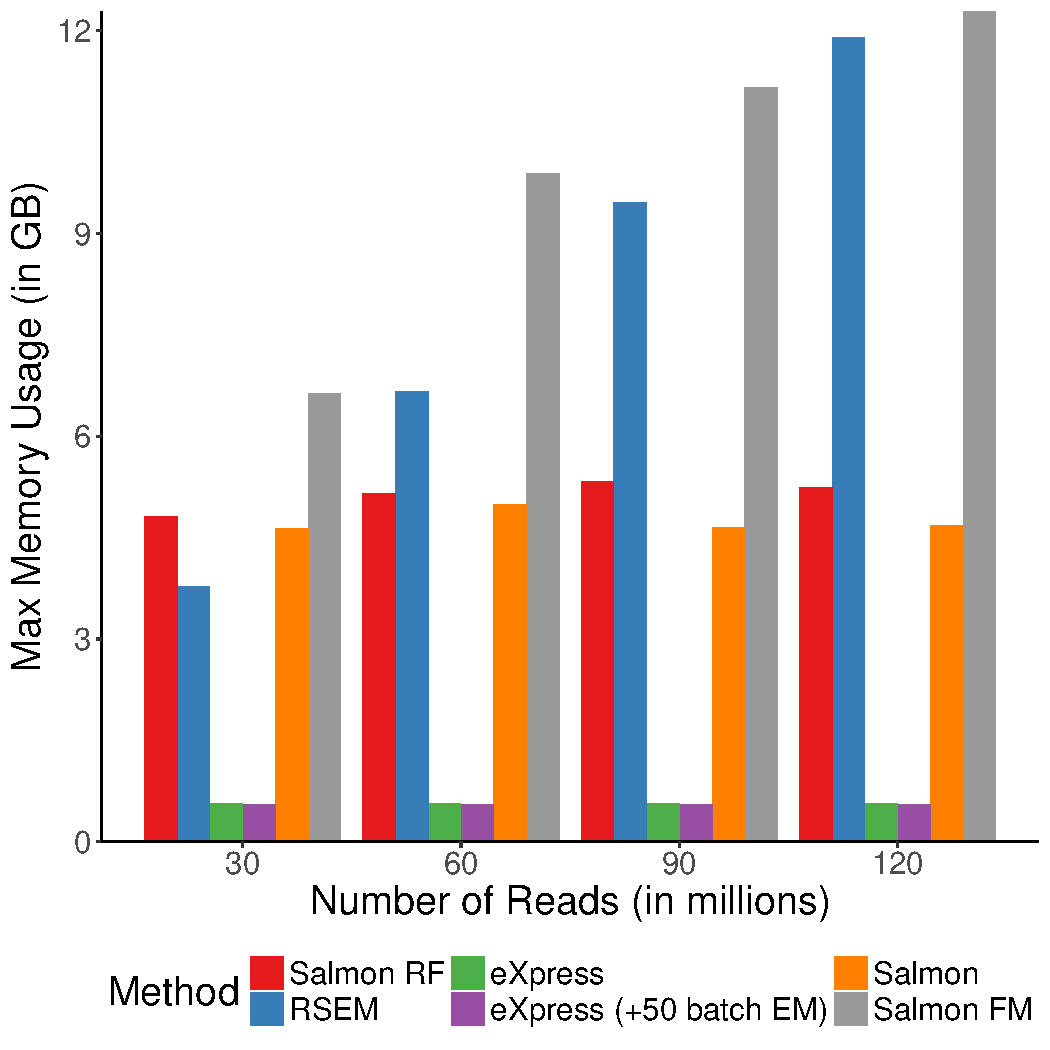
\includegraphics[width=0.5\textwidth]{Figures/DDFact/memory_sim}
   \caption[Maximum runtime of different methods]{Maximum memory used by each method 
   while running on input read files of sizes from 30M paired-end read counts to 120M. 
   Memory usage of \rsem and \salfm keeps increasing linearly by the read input counts 
   since those tools provide full fidelity by storing  conditional probabilities of 
   each fragment-transcript pair. \salmon and \salrf keep memory usage constant by using 
   the notion of equivalence classes and clustering reads together. \express and \expressEM 
   also have constant memory usage, which is the lowest among all methods.  However, this 
   low memory usage is obtained at the expense re-loading all the alignments from the input 
   \texttt{BAM} file in each iteration of the EM algorithm.  This induces a considerable 
   runtime burden, per EM-round, compared to other tools as displayed 
   in~\cref{supfigure:time_anal}.}
   \label{supfig:memory_anal}
\end{figure}

\begin{figure}[h]
   \centering
   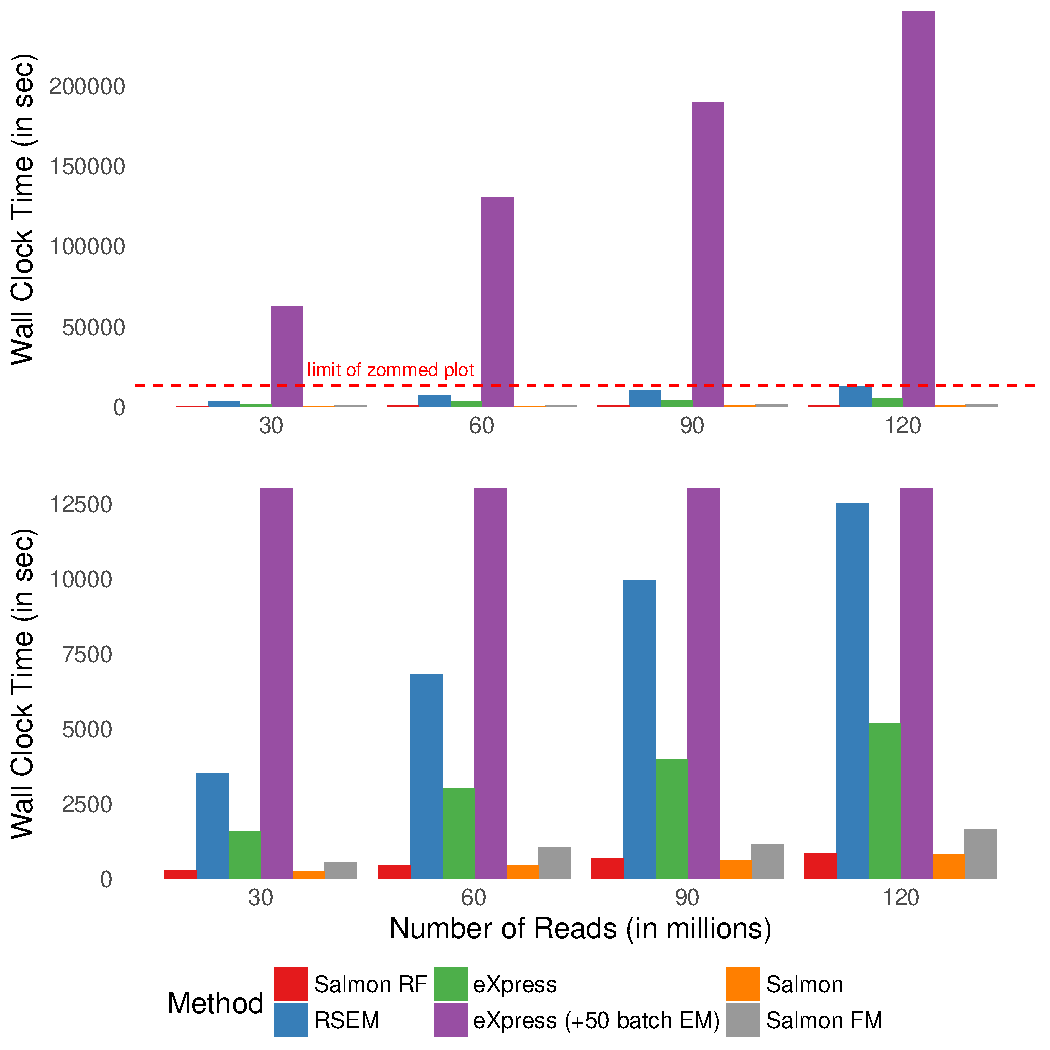
\includegraphics[width=0.5\textwidth]{Figures/DDFact/times_sim}
   \caption[Total wall-clock time of different methods]{Total wall-clock time of each 
   method as the number of paired-end reads is scaled from 30M to 120M. All methods receive 
   the alignment \texttt{BAM} file as pre-computed input (i.e., alignment time is not 
   considered in these evaluations). \salrf is as fast as \salmon, and both are twice as 
   fast as \salfm which is the result of the reduced complexity of their batch EM rounds. 
   \rsem, which also uses the full model in each iteration, takes longer than the \salmon 
   variants. \textbf{Note}, unlike other methods, \express does not scale beyond  2 threads 
   (when bias correction is disabled).  Thus, we have placed an asterisk next to \express in 
   the legend here to designate that the results should not be taken as a direct comparison 
   to the other methods (which are using 16 threads). \expressEM is considerably slower 
   than other methods since \express is a constant-memory algorithm that iterates through the 
   entire alignment \texttt{BAM} file (reading the alignments from disk) once per EM round.}
   \label{supfigure:time_anal}
\end{figure}


Though we observe an improvement for \salmonrf and \salmonfm over \salmon and
especially \salmonu in this case, we note that it is relatively small in scale.
This is because, while the aggressive \cb factorizations do give up information,
common expression patterns may not be complex or difficult enough to be greatly
affected by the lossy factorization of the likelihood. Also, however, these
aggregate metrics are computed over the entire transcriptome, and so,
difficulties of these factorizations in deconvolving particularly complex
scenarios may become lost in the noise of the vast number of good predictions.

\begin{table} \centering
    \begin{tabular}{lrrrr}
    \toprule
    {} & MARD-all   & Spearman-all & MARD-subset & Spearman-subset \\
    \midrule
    \salu & \num{0.23859} & \num{0.80022} & \num{0.46048} & \num{0.56145} \\
    \salmon & \num{0.22272} & \num{ .81307} & \num{0.43192}  & \num{0.57537} \\
    \salrf & \num{0.21433} & \num{0.82507} & \num{0.41232} & \num{0.64425} \\
    \salfm  & \num{0.21409} & \num{0.82506} & \num{0.41058} & \num{0.64657} \\
    \express & \num{0.28864} & \num{0.77775} & \num{0.52639} & \num{0.54326} \\
    \expressEM & \num{0.22711} & \num{0.82748} & \num{0.47694} & \num{0.59295} \\
    \rsem & \textbf{\num{0.21241}} & \num{0.81955} & \num{0.40791} & \num{0.65387} \\
    \bottomrule
    \end{tabular}
    \captionof{table}[Accuracy of quantification of synthetic reads]
    {Spearman correlation and MARD of quantification results compared to true abundances 
    for synthetic data on all transcripts (MARD-all and Spearman-all), and the subset of 
    transcripts (MARD-subset and Spearman-subset) where \emph{RSEM}'s ARD is 
    in $\left[0.25, 0.75\right]$.}
    \label{tab:fidelity}
\end{table}


\begin{table} \centering
    \begin{tabular}{lrrrr}
    \toprule
    {} & MARD-all   & Spearman-all & MARD-subset & Spearman-subset \\
    \midrule
    \salu & \num{0.23859} & \num{0.80022} & \num{0.46048} & \num{0.56145} \\
    \salmon & \num{0.22272} & \num{0.81307} & \num{0.43192}  & \num{0.57537} \\
    \salrf & \textbf{0.214} & \textbf{0.825} & \textbf{0.412} & \textbf{0.644} \\
    \salfm  & \textbf{0.214} & \textbf{0.825} & \textbf{0.411} & \textbf{0.647} \\
    \express & \num{0.28864} & \num{0.77775} & \num{0.52639} & \num{0.54326} \\
    \expressEM & \num{0.22711} & \textbf{0.827} & \num{0.47694} & \num{0.59295} \\
    \rsem & \textbf{0.212} & \textbf{0.820} & \textbf{0.408} & \textbf{0.653} \\
    \bottomrule
    \end{tabular}
    \captionof{table}[Accuracy of quantification of synthetic reads]{Spearman correlation 
    and MARD of quantification results compared to true abundances for synthetic data on 
    all transcripts (MARD-all and Spearman-all), and the subset of transcripts 
    (MARD-subset and Spearman-subset) where \emph{RSEM}'s ARD is in 
    $\left[0.25, 0.75\right]$.}
    \label{tab:fidelity1}
\end{table}

\begin{figure}[t]
    \centering
    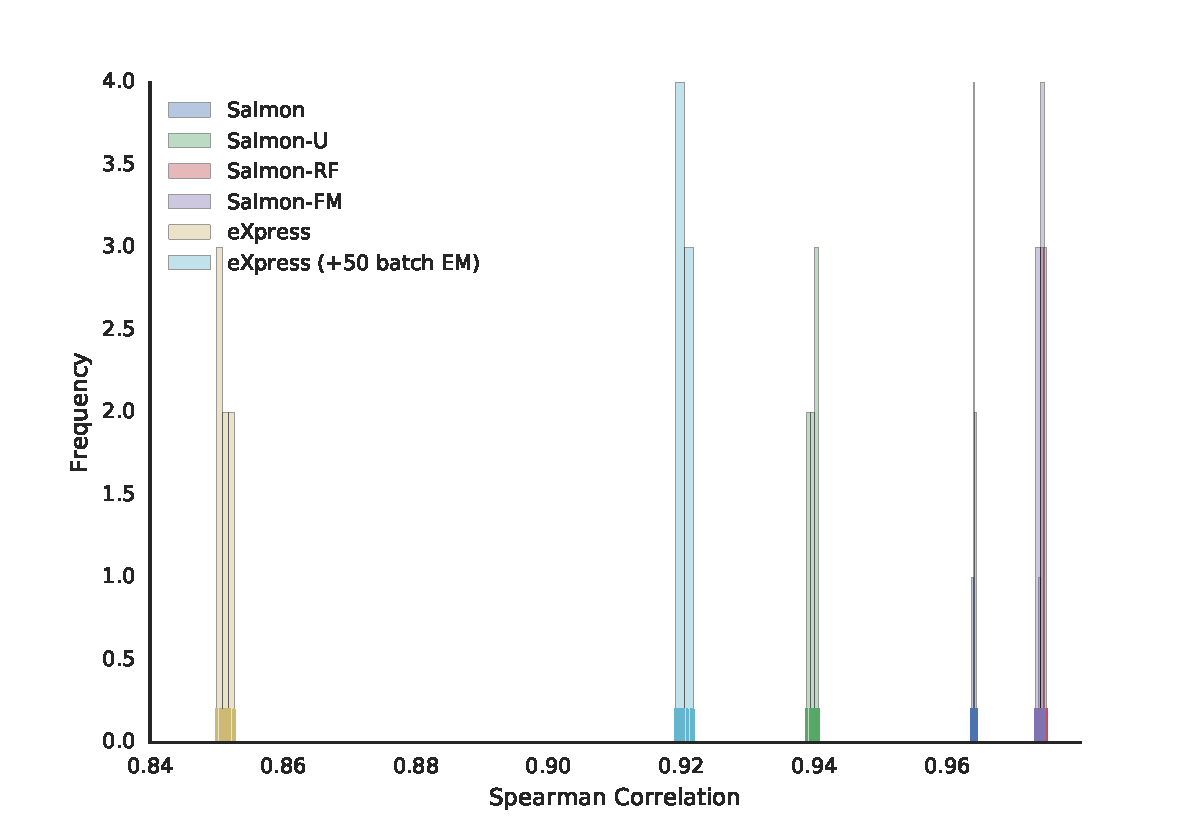
\includegraphics[width=0.9\textwidth]{{{Figures/DDFact/Patro.287.fig.5a}}}
    \caption[The accuracy of quantification of experimental data - Spearman Correlation]
        {The Spearman correlation of transcripts abundance estimations with
        \rsem results reveals that \salfm is highly correlated with \rsem. Very
        similar correlation with \rsem is observed by the proposed data-driven
        factorization, \salrf. \salmon displays a lower correlation than \salrf,
        but a higher correlation than \salu. The variants of \express show a lower
        correlation than \salu, with the offline EM iterations increasing
        \express' correlation considerably.}
    \label{fig:exp_spear}
\end{figure}
%\qquad
\begin{figure}[t]
    \centering
    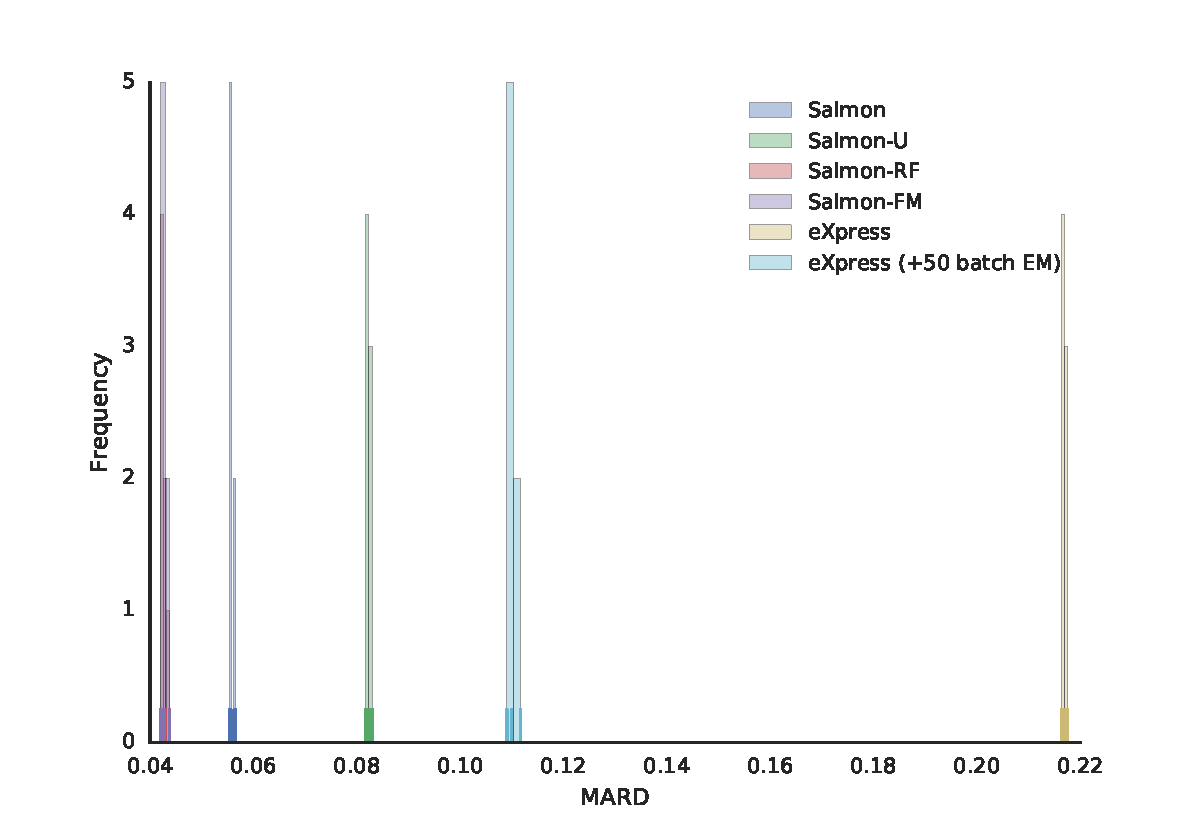
\includegraphics[width=0.9\textwidth]{{{Figures/DDFact/Patro.287.fig.5b}}}
    \caption[The accuracy of quantification of experimental data - MARD]
    {Comparing the MARD of estimated transcript fragment counts with
    respect to \rsem results shows similar trend to that observed with the
    Spearman correlations;i.e., \salfm has the least error rate using RSEM
    abundances as the truth while \salrf perform equally well.  \salmon exhibits
    a lower MARD than \salu, which is followed by both variants of \express.}
    \label{fig:exp_mard}
%   \caption[Accuracy of quantifications with different versions of salmon 
%   with the experimental reads]
%   {Comparison of the transcript abundances in different versions of salmon 
%   on the experimental data with 7 technical 
%   replicates and using rsem abundance estimates as the ground truth.}
\end{figure}

To focus on the more difficult cases, we computed our accuracy metrics on a
subset of the simulated data. Specifically, retaining the original abundance
estimates over the entire transcriptome, we restricted our analysis to those
transcripts for which \rsem obtained an ARD between $0.25$ and $0.75$. The
motivation for choosing these values is to discard the particularly ``easy'' to
quantify transcripts (where the \fm is likely neither necessary nor particularly
helpful) as well as the ``hopeless'' transcripts (those where the inference
exhibits significant error even under the reference implementation of the \fm).
The results of this analysis are shown in second two columns of~\Cref{tab:fidelity} 
(MARD-subset and Spearman-subset). While the trend is similar to that observed on 
the full data, the difference between methods (and the impressive performance 
of \salmonrf) becomes more clear. Specifically, we observe that \salmon outperforms 
\salmonu, but this time the gap between \salmon and \salmonrf, \salmonfm and \rsem
is larger. This is most likely because this particular subset of transcripts 
presents a more difficult inference challenge, where the conditional probabilities 
provide useful evidence. In the case of these transcripts, running the EM algorithm 
until convergence seems particularly important, as we observe that \express (and even
\expressEM) trail the other methods, especially in terms of the MARD. This makes
it evident that further refinement of the abundance estimates (i.e. more rounds
of the EM) over a representation of the data encoding conditional fragment
probabilities (as done in \rsem, \salfm and \salrf) is necessary to obtain
improved accuracy on these transcripts.

\label{sec:experimental}

\begin{table}
\centering
\begin{tabular}{lrr}
    % {
    % lS[table-format=7]S[table-format = 7]S[table-format = 7]S[table-format = 9]
    % }
\toprule
{} &          $\#$ eq. classes &     $\#$ hits \\
\midrule
\salu & 438393& 5986371\\
\salmon  & 438393& 5986371 \\
\salrf &625638 & 8212669\\
\salfm & 29447710& 103663423\\
\bottomrule
% \toprule
% {} &          \salu &     \salmon &        \salrf &         \salfm \\
% \midrule
% \# eq. classes &438393  &438393  &625638 &29447710 \\
% \# hits                           &5986371 &5986371 &8212669 &103663423\\
% \bottomrule
\end{tabular}
\caption{The number of equivalence classes and hits, in the
  simulated data, under different likelihood factorizations.}
\label{tab:performance_table}
\end{table}


We further investigate the performance of tools in non-alignment mode as well. Spearman 
correlation and MARD of transcript quantification with different tools on RSEM simulated 
data is presented in~\Cref{tab:exp-mapping,tab:exp-mapping_select}. 

\begin{table}
\centering
\begin{tabular}{lrrrr}
    \toprule
    {} &    \kallisto &     \salmon &        \salrf &          \salfm \\
    \midrule
      MARD  &  \num{0.23067}  &  \num{0.22737}  &  \num{0.22673} &  \num{0.22668}  \\
      Spearman Correlation & \num{0.8053} & \num{0.81003} & \num{0.81078} & \num{0.81105}\\
    \bottomrule
    \end{tabular}
    \caption[The accuracy of estimations of all transcripts in ``mapping'' mode]
    {The Spearman correlation and MARD of
    estimations by different tools in ``mapping'' mode on synthetic data
    simulated by RSEM-sim as described in~\cref{res:largescale}. We observe that, when
    using mappings instead of full alignments, the factorization being used has
    a smaller effect (an observation worthy of further consideration in future work). 
    Still, we observe that \salmon performs slightly better
    than \kallisto (which has a factorization akin to \salu), 
    while \salrf and \salfm perform best.\label{tab:exp-mapping}}
\end{table}

\begin{table}
\centering 
\begin{tabular}{lrrrr}
    \toprule
    {} &    \kallisto &     \salmon &        \salrf &          \salfm \\
    \midrule
      MARD  &  \num{0.44136}  & \num{0.43301}  &  \num{0.42957} &  \num{0.42925}  \\
      Spearman Correlation  & \num{0.59137} &  \num{0.60262} &  \num{0.61445} & \num{0.6139} \\
    \bottomrule
    \end{tabular}
    \caption[The accuracy of estimations of difficult transcripts in ``mapping'']
    {The Spearman correlation and MARD of the estimates of different methods in mapping 
    mode on synthetic data simulated by RSEM-sim. These metrics are computed only over 
    the ``difficult'' transcripts---the set of transcripts for which \rsem achieves 
    ARD values between 0.25 and 0.75. \label{tab:exp-mapping_select}}
\end{table}

\subsection{Transcriptome-wide analysis on experimental data}

Finally, we explore the effect of our data-driven factorization method with the
different versions of \salmon using experimental data from the SEQC(MSEQ-III)
consortium~\citep{seqc2014comprehensive} (NCBI GEO accession \texttt{SRR1215996}
- \texttt{SRR1217002}). Specifically, the library is prepared on Universal Human
Reference RNA (UHRR) from Stratagene and ERCC Spike-In controls and consists of
$\sim$11M $100$bp, paired-end reads sequenced on an Illumina HiSeq 2000
platform. The experiment consists of seven replicates with the same flowcell and
barcodes but on different lanes.

As defined previously in~\cref{res:smallscale} we compare the performance of
\salmon, \salfm, \salrf, \salu, \express, \expressEM with \rsem. However, unlike
in previous sections, here, we lack a ground truth. Thus, we measure the
accuracy of each method on the estimated number of reads, treating \emph{RSEM}'s
estimations of the number of reads for each transcript (which is observed to be
among the most accurate on synthetic data in previous sections) as the truth. We
perform a comparison across all seven replicates and consider the Spearman
correlation and MARD metrics. Since these are technical replicates, we expect
the performance over each replicate to be very similar, though we plot the
results as a distribution in~\Cref{fig:exp_spear} and~\Cref{fig:exp_mard}. The
results on experimental data follow the same trend as we observed on synthetic
data. That is, \salfm correlates well with \rsem (as expected) because of the
availability of full fragment level transcript probabilities. Likewise, we again
observe that our proposed data-driven factorization method, \salrf, performs
essentially the same as the \fm. Both of these methods agree more closely with
\rsem than does \salmon, and again, \salmonu, ignoring all fragment-level
conditional probabilities, is further from \emph{RSEM}'s results. The number of
equivalence classes for each factorization are shown
in~\Cref{tab:performance_table_real}. We also observe that \express, in its
default mode, performs most differently from \rsem of the methods we considered.
As expected, running additional rounds of the batch EM (\expressEM) increases
the similarity of \express' estimations with those of \rsem; though it is still
less similar than the other methods.
\label{res:expdata}

\section{Conclusion}
\begin{table}\centering
    \begin{tabular}{lS[table-format=7]S[table-format=7]S[table-format=7]S[table-format=9]}
    \toprule
    {} &          \salu &     \salmon &        \salrf &         \salfm \\
    \midrule
    \# eq. classes &  427611 &   427611    &  624340 &  9077708 \\
    \# hits     & 5737414 & 5737414  &   8318638 & 50325595 \\
    \bottomrule
    \end{tabular}
    \caption[The number of equivalence classes and hits]
    {The number of equivalence classes and hits, in the
    experimental data, under different likelihood factorizations.}
    \label{tab:performance_table_real}
\end{table}


While compatibility-based equivalence class
factorizations~\citep{Turro2011Haplotype,Nicolae2011Estimation,Patro2014Sailfish,
Srivastava2016rapmap,Bray2016Kallisto}
have paved the way in terms of substantially improving the efficiency of the
iterative optimization procedures used for transcript-level quantification from
RNA-seq data, they nonetheless make sacrifices in modeling fidelity to achieve
this. While these methods generally perform adequately in terms of
transcriptome-wide assessments, there are still important situations in which
their compatibility-centric factorization of the underlying likelihood function
discards information that can be important for accurate abundance estimates.
\salmon~\citep{Patro2017Salmon} uses a dual-phase inference algorithm that
allows it to recover some of the information discarded by other approaches. It
improves upon the approximate factorization of the full likelihood function by
incorporating a notion of \emph{rich} equivalence classes of fragments. In some,
but not all cases, this improved factorization is sufficient to recover the lost
accuracy of the full model.

In this chapter, we have introduced a data-driven factorization of the likelihood
function that makes use of \salmon's dual-phase inference algorithm (\salmonrf).
We have shown that this improved factorization is able to match the accuracy of
the \fm while still maintaining a reduced representation that is orders
of magnitude smaller than the total number of fragment alignments.

We believe that this data-driven factorization represents the right tradeoff
between efficiency and accuracy. Specifically, it demonstrates an almost
indistinguishable sacrifice in efficiency beyond the factorization already
employed by \salmon (which, itself, is similar in size to those employed by
\mmseq, \sailfish and \kallisto), while producing no perceptible loss in
accuracy compared to the full per-fragment likelihood function used by \rsem and
similar methods.

In this chapter, we have focused on the effect that the adopted factorization of
the likelihood function can have on the ability of a method to accurately
estimate transcript abundance. However, we note that there still remain small
but interesting differences between methods that employ alignment and those that
rely on mapping (i.e., quasi-mapping or pseudoalignment). Fully exploring the
nature of these differences, and how they interact with the factorizations
proposed herein, is an interesting direction for future work.

Finally, while we have investigated the effect different factorizations have on
maximum likelihood estimates, fully-exploring the effect they have in estimating
the variance of these estimates (e.g., via bootstrapping) or even in estimating
the full posterior distribution of abundances (e.g., via Gibbs sampling) is
another interesting direction for future work.\\